\chapter{Implementation: Quantum Systems}

For a quantum system to be studied on the computer it is necessary to 
make a distinction for what defines the system. One must therefore undergo the
mathematical procedure of defining a finite basis sets that defines the 
quantum system under scrutiny when dealing with the electronic problem. 

Here we present the \lstinline{quantum_system} python module, designed to 
provide basis sets for one- and two-dimensional quantum dots. The two-dimensional 
quantum dot can also be modelled with a constant, homogeneous magnetic field; and 
as a double quantum dot. 
Moreover, the module includes an option for constructing a custom system which can 
be interfaced with popular quantum chemistry packages \lstinline{PySCF}\cite{PYSCF} 
and \lstinline{Psi4}\cite{parrish2017psi4}.

The \lstinline{quantum_system} module can installed from github with \lstinline{pip}
by the following command,
\begin{lstlisting}[language=bash]
pip install git+https://github.com/Schoyen/quantum-systems.git
\end{lstlisting}
The same task can of course be accomplished by more commands,
\begin{lstlisting}[language=bash]
git clone https://github.com/Schoyen/quantum-systems.git
cd quantum-systems
pip install .
\end{lstlisting}

\noindent
--------------\\
NOTE: not sure the part below here is necessary. Maybe just link to web page 
documentation? If it is done, that is.. \\
--------------

It can be useful to install the module to a separate environment. We have made this 
possible through \lstinline{conda},
\begin{lstlisting}[language=bash]
conda environment create -f environment.yml
conda activate quantum-systems    
\end{lstlisting}

\section{Quantum Dots}

In reality, quantum dots are nanometre-sized structures made of semiconductor materials.
Theoretically, quantum dots are easy to model by harmonic oscillator potential and in practice
they are relativelty easy to manufacture in a laboratory. This doubly
theoretical-experimental benefit has made quantum dots a popular area of study. Moreover so 
because of their wide area of apllications.

The possible applications of quantum dots are many. Coupled single-electron quantum dots 
could potentially be used as harware elements in quantum computers, i.e.
qubits\cite{loss1998quantum}; quantum dots also promise to increase the efficiency of 
photvoltaic solar cells; and they have already found use in cellular imaging in biology.
Reimann and Manninen\cite{reimann2002electronic} has written an outstandingly
thorough review on quantum dots, covering their varied types of fabrication, theoretical
methods common in their study and vast ocean of applications.

The usefulness and relative theoretical ease of modelling warrants the study of quantum dots.
Herein, several classes have been implemented in order to construct basis sets modelling 
quantum dots in both one and two dimensions. These basis sets models \emph{bound} systems
as the common harmonic oscillator-type potentials that are used have the characteristics of 
infinite quantum wells. 

\subsection{One Dimension}

This is perhaps one of the simplest of all quantum mechanical 
models, being studied ad nauseum in everyones introductory quantum 
mechanics course. The one-body part of the Hamiltonian for the one-dimensional quantum 
harmonic oscillator is,
\begin{equation}
    \label{eq:1d_ho_hamiltonian}
    \hat{h} = \frac{\hat{p}^2}{2m} + \frac{1}{2}m \omega^2\hat{x}^2.
\end{equation}
The potential, $\hat{v} = \frac{1}{2}m \omega^2\hat{x}^2$, forms the well known 
parabolig curve. In a general one-dimensional system, this potenation could 
readily be exchanged for something else. For instance that of the 
\emph{double well},
\begin{equation}
    \hat{v} = \frac{1}{2} m \omega^2
        \left(\hat{x}^2 + \frac{1}{4}l^2 - l |\hat{x}|\right),
\end{equation}
where $l$ is the width of a barrier in the middle of the parabolic 
potential.

In atomic units we can set $\hbar = m = 1$. Substituting for the 
momentum operator, $\hat{p} = \hat{-i\hbar (\partial / \partial x)}$, gives us 
\begin{equation}
    \label{eq:1d_hamiltonian}
    \hat{h} = - \frac{1}{2} \frac{\partial^2}{\partial x^2} + \hat{v}.
\end{equation}
The second-order derivate can be approximated by the central difference 
formula for some function $f(x)$, yielding
\begin{equation}
    f''(x) = \frac{f(x + dx) - 2f(x) +f(x - dx)}{dx^2},
\end{equation}
for some small $dx$. This means that we approximate the Hamilton 
operator of the system (\autoref{eq:1d_hamiltonian}) by a matrix,
\begin{equation}
    h^p_q =  \begin{pmatrix}
    1/dx^2 + v_1 & -1/2dx^2 & \ddots & & & \\
    -1/2dx^2 & 1/dx^2 + v_2 & -1/2dx^2 & \ddots & & \\
    \ddots & -1/2dx^2 & 1/dx^2 + v_3 & -1/2dx^2 & \ddots & \\
    & \ddots & \ddots & \ddots & \ddots & \ddots \\
    & & \ddots & -1/2dx^2 & 1/dx^2 + v_{n-1} & -1/2dx^2 \\
    & & & \ddots & -1/2dx^2 & 1/dx^2 + v_n
    \end{pmatrix},
\end{equation}
and we have thus transformed the time-independent Schrödinger equation
\begin{equation}
    \hat{h} \ket{n} = \epsilon \ket{n},
\end{equation}
into a matrix equation which is easily representable and solvable on a computer, where $n$ is 
the number of points used to numerically represent the wavefunciton 
and Hamiltonian mateix representation. This is done with some generic 
eigenvalue solver, for instance \lstinline{numpy.linalg.eigh}.
The eigen functions provide the foundations for the single-particle functions.

Since we would like to model interaction between particles we need something more,
than just a numerical representation of the one-body operator. We therefore need to 
compute coulomb interaction, in the form of an integral. This is done in
several steps, starting with an ``inner intergral'' over all all space 
and two and two single-particle functions,
\begin{equation}
   u^q_s = \int \phi_q(x_1) \frac{\alpha}{(x_1-x_2)^2 + 2a^2}  \phi_s(x_2) dx,
\end{equation}
where $a$ and $\alpha$ are parameters that are necessary to include for this integral 
to be calculable.
Numerically, this part is divided into two functions in our python implementation,
\begin{python}
def _shielded_coulomb(x_1, x_2, alpha, a):
    return alpha / np.sqrt((x_1 - x_2) ** + a ** 2)

def _compute_inner_integral(spf, l, num_grid_points, grid, alpha, a):
    inner_integral = np.zeros((l, l, num_grid_points), dtype=np.complex128)

    for q in range(l):
        for s in range(l):
            for i in range(num_grid_points):
                inner_integral[q, s, i] = _trapz(
                    spf[q]
                    * _shielded_coulomb(grid[i], grid, alpha, a)
                    * spf[s],
                    grid,
                )

    return inner_integral
\end{python}
The inner orbital is then used in the computation in the orbial integral,
\begin{equation}
    w^{pq}_{rs} = \int \phi_p u^q_s \phi_r dx,
\end{equation}
which numerically is implemented as follows,
\begin{python}
def _compute_orbital_integrals(spf, l, inner_integral, grid):
    u = np.zeros((l, l, l, l), dtype=np.complex128)

    for p in range(l):
        for q in range(l):
            for r in range(l):
                for s in range(l):
                    u[p, q, r, s] = _trapz(
                        spf[p] * inner_integral[q, s] * spf[r], grid
                    )

    return u
\end{python}

Each integral is solved by the trapezoidal scheme,
\begin{python}
def _trapz(f, x):
   n = len(x)
   delta_x = x[1] - x[0]
   val = 0

   for i in range(1, n):
       val += f[i - 1] + f[i]

   return 0.5 * val * delta_
  
\end{python}

Needless to say, computing the coulomb integrals is one of the more compute-heave tasks,
and we therefore make great use of just-in-time compulation from the \lstinline{numba} 
module for python.

A full representation of the one-dimensional quantum dot (oscillator) class is provided 
below,
\begin{tcolorbox}
    {\fontfamily{cmss}\selectfont
    \textbf{class} quantum\_systems.\textbf{ODQD}

    \hspace{1em}(\emph{n}, \emph{l}, \emph{grid\_length}, \emph{num\_grid\_points}, 
    \emph{a=$0.25$}, \emph{alpha=$1.0$})

    \vspace{1em}
    Create One-Dimensional Quantum Dot basis set.
    \vspace{1em}

    \textbf{Parameters}

    \hspace{2em}\textbf{n}(\emph{int}) Number of electrons
    
    \hspace{2em}\textbf{l}(\emph{int}) Number of spinorbitals
    
    \hspace{2em}\textbf{grid\_length}(\emph{int, float}) Space over which to 
        construct wavefunction.
    
    \hspace{2em}\textbf{num\_grid\_points}(\emph{int, float}) Number of 
        points for construction of wavefunction.

    \hspace{2em}\textbf{a}(\emph{float, default $0.25$}) Coulomb screening parameter.
    
    \hspace{2em}\textbf{alpha}(\emph{float, default $1.0$}) Coulomb strength parameter. 

    \vspace{1em}
    \textbf{Attributes}

    \hspace{2em} \textbf{h}
    One-body matrix 
    \textbf{Type} \emph{np.array}
    
    \hspace{2em} \textbf{f}
    Fock matrix
    \textbf{Type} \emph{np.array}

    \hspace{2em} \textbf{u}
    Two-body matrix
    \textbf{Type} np.array

    % \hspace{2em} \textbf{o}
    % Occupied orbital indices
    % \textbf{Type} \emph{Slice} object

    % \hspace{2em} \textbf{v}
    % Virtual orbital indices
    % \textbf{Type} \emph{Slice} object

    \vspace{1em}
    \textbf{Methods}

    \hspace{2em} \textbf{setup\_system}(\emph{Potential=None})
        \begin{adjustwidth}{4em}{}
        Must be called in order to compute basis functions. The method will 
        revert to regular harmonic oscillator potential with $\omega=0.25$
        if no potential has been provided.
        Optional potentials include one-dimensional double well potentials.           
        \end{adjustwidth}
   
    \hspace{2em} \textbf{contruct\_dipole\_moment}()
        \begin{adjustwidth}{4em}{}
        Constructs dipole moment. This method is called by
        \textbf{setup\_system}(). Necessary when constructing custom systems with 
        time development.
        \end{adjustwidth}
    }
\end{tcolorbox}


\subsection{Two Dimensions}

The one-body part of the Hamiltonian for a two-dimensional quantum dots is almost
identical to the one-body part for a one-dimensional quantum dot. In cartesian
coordinates we simple include a $y$ in the potential as well as an $x$, but mostly 
because we have analytical expressions for the Coulomb integrals in polar
coordinates\cite{anisimovas1998energy}, we write the one-body operators in 
polar coordinates as well with $\hat{r}^2 = \hat{x}^2 + \hat{y}^2$,
\begin{equation}
    \hat{h} = \frac{\hat{p}^2}{2m} + \frac{1}{2}m\omega^2\hat{r}^2
        = - \frac{\hbar^2}{2m}\left(
            \frac{\partial^2}{\partial r^2}
            + \frac{1}{r} \frac{\partial}{\partial r}
            + \frac{1}{r^2} \frac{\partial^2}{\partial \theta^2}
        \right)
        + \frac{1}{2}m\omega^2\hat{r}^2.
\end{equation}

The wavefunctions for a two-dimensional harmonic oscillator can be
written
\begin{equation}
    \label{eq:2d_ho_eigenstate}
    \phi(r,\theta) = N_{nm} R_{nm}(r) Y_m(\theta) = N_{nm} (ar)^{\abs{m}} L_n^{\abs{m}}(a^2r^2)
        e^{-a^2r^2/2} e^{im\theta},
\end{equation}
where $a=\sqrt{m\omega/\hbar}$ si the Bohr radius, $L^{\abs{m}}_n$ is 
the associated Laguerre polynomials, $n$ and $m$ are the principal and
the azimutal quantum numbers respectively\footnote{There is usually another quantum 
number called the magnetic quantum number. Because of our restriction to two dimensions,
this quantum number does not appear. In three dimensions we would usually denote the azimuthal
quantum number by $l$ and the magnetic quantum number by $m$ or $m_l$. A fourth quantum 
number is the spin projection quantum number commonly written $m_s$.}, and $N_{nm}$ is a normalisation 
factor given by,
\begin{equation}
    N_{nm} = a\sqrt{\frac{n!}{\pi(n + \abs{m})!}}.
\end{equation}


The energy eigenvalues of a two-dimensional harmonic oscillator is given by 
\begin{equation}
    \epsilon_{nm} = \hbar\omega(2n + \abs{m} + 1).
\end{equation}
It is very beneficial that such a nice expression exists, because the one-body 
matrix elements of a harmonic oscillator is simply,
\begin{equation}
    \bra{\phi_p}\hat{h}\ket{\phi_q} = \hat{h}^p_q = \epsilon_p \delta^p_q.
\end{equation}
These matrix elements encompass both the kinetic energy operator matrix element and 
potential energy matrix element. If we were dealing with completely none-interacting 
particles not much more would be nedded.
We see, however, that this form of one-body matrix elements necessitates a mapping from 
the general coordinates $p,q$, as used above, and the quantum numbers $n,m$.

This functionality $(n,m)\mapsto p$ is 
achieved by the following python function
\begin{python}
def get_index_p(n, m):
    num_shells = 2 * n + abs(m) + 1

    previous_shell = 0
    for i in range(1, num_shells):
        previous_shell += i

    current_shell = previous_shell + num_shells

    if m == 0:
        if n == 0:
            return 0

        p = previous_shell + (current_shell - previous_shell) // 2

        return p

    elif m < 0:
        return previous_shell + n

    else:
        return current_shell - (n + 1)
\end{python}
It will also be necessary to map back $p\mapsto(n,m)$,
\begin{python}
def get_indices_nm(p):
    n, m = 0, 0
    previous_shell = 0
    current_shell = 1
    shell_counter = 1

    while current_shell <= p:
        shell_counter += 1
        previous_shell = current_shell
        current_shell = previous_shell + shell_counter

    middle = (current_shell - previous_shell) / 2 + previous_shell

    if (current_shell - previous_shell) & 0x1 == 1 and abs(
        p - math.floor(middle)
    ) < 1e-8:
        n = shell_counter // 2
        m = 0

        return n, m

    if p < middle:
        n = p - previous_shell
        m = -((shell_counter - 1) - 2 * n)

    else:
        n = (current_shell - 1) - p
        m = (shell_counter - 1) - 2 * n

    return n, m
\end{python}

An important difference between the one-dimensional quantum dot and a two-dimensional 
quantum dot is that in the latter we have energy degeneracies of the eigenstates.
This is illustrated in \autoref{fig:2d_basis_states}. In this figure we have included 
a spin-up and a spin-down state for each $n,m$-state. This spin feature is not in any way 
included in \autoref{eq:2d_ho_eigenstate}, but we may represent the spin condition by
including it in the orthonormality conditions of the wavefunctions,
\begin{equation}
    \braket{n_1m_1\sigma_1}{n_2m_2\sigma_2} 
    = \delta_{n_1n_2}\delta_{m_1m_2}\delta_{\sigma_1\sigma_2},
\end{equation}
where $\sigma$ is the spin.

\begin{figure}
    \begin{center}
        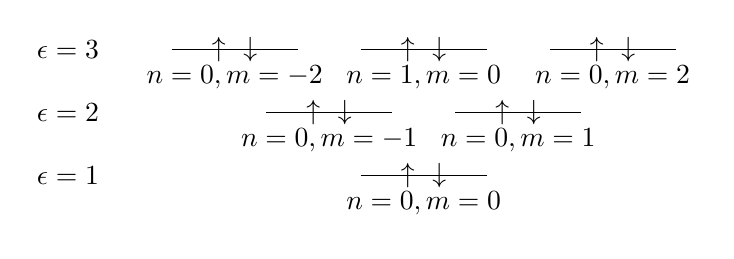
\begin{tikzpicture}[scale=0.8]
            \begin{scope}
                \foreach \i in {1, 2, 3} {
                    \draw(-1, \i - 1) node[anchor=east]
                    {$\epsilon = \i$};
                }

                % Highest energy level
                \foreach \i in {0, 3, 6} {
                    \draw (\i, 2) -- (\i + 2, 2);
                    \node at (\i + 0.75, 2) {$\uparrow$};
                    \node at (\i + 1.25, 2) {$\downarrow$};
                }
                \node[below, inner sep=.2cm] at (1, 2)
                {$n = 0, m = -2$};
                \node[below, inner sep=.2cm] at (4, 2)
                {$n = 1, m = 0$};
                \node[below, inner sep=.2cm] at (7, 2)
                {$n = 0, m = 2$};

                % Middle energy level
                \foreach \i in {1.5, 4.5} {
                    \draw (\i, 1) -- (\i + 2, 1);
                    \node at (\i + 0.75, 1) {$\uparrow$};
                    \node at (\i + 1.25, 1) {$\downarrow$};
                }
                \node[below, inner sep=.2cm] at (2.5, 1)
                {$n = 0, m = -1$};
                \node[below, inner sep=.2cm] at (5.5, 1)
                {$n = 0, m = 1$};

                % Lowest energy level
                \draw (3, 0) -- (5, 0);
                \node at (3 + 0.75, 0) {$\uparrow$};
                \node at (3 + 1.25, 0) {$\downarrow$};
                \node[below, inner sep=.2cm] at (4, 0)
                {$n = 0, m = 0$};
            \end{scope}
        \end{tikzpicture}
    \end{center}
    \caption{In this plot we see the energy degeneracy of the
    lowest three energy levels in the two-dimensional quantum dot.
    Each arrow representes a spin up or a spin down state with the
    quantum numbers $n$ and $m$ as listed below. This pattern goes
    on indefinitly with the addition of one bar (two oscillators)
    per level.}
    \label{fig:2d_basis_states}
\end{figure}

Because the electrons we will be studying are interacting, we need two-body matrix elements 
as well. The analytical formula for the Coulomb interaction integrals, provided by Anisimovas and 
Matulis\cite{anisimovas1998energy} is
\begin{equation}
    \begin{aligned}
        \langle \phi_1\phi_2| \hat{W} | \phi_3\phi_4 \rangle =& 
        \delta_{s_1, s_4} \delta_{s_2, s_3} \delta_{m_1 + m_2, m_3 + m_4}
        \Big[\prod_{i=1}^4 \frac{n_i!}{(|m_i| + n_i)} \Big]^{1/2}
        \sum_{(4)j=0}^n \frac{(-1)^{j_1+j_2+j_3+j_4}}{j_1!j_2!j_3!j_4!} \\
        &\times \Big[\prod_{i=1}^n {n_i + |m_i| \choose n_i + j_i} \Big]
        \frac{1}{2^{(G+1)/2}} \sum_{(4)l=0}^\gamma (-1)^{\gamma_2 + \gamma_3 - l_2 - l_3} \\
        &\times \delta_{l_1 + l_2, l_3 + l_4} \Big[\prod_{i=1}^4 {\gamma_i \choose l_i} \Big] 
        \Gamma\Big(1 + \frac{L}{2} \Big)\Gamma\Big(\frac{G - L + 1}{2}\Big).
    \end{aligned}
\end{equation}
The symbols $j_i$ are integer summation indices (regular indices) running from $0$ to $n_i$.
The symbols $\gamma_i$ stand for numbers,
\begin{align*}
\gamma_1 &= j_1 + j_4 + (|m_1| + m_1)/2 + (|m_4| - m_4)/2 \\
\gamma_4 &= j_1 + j_4 + (|m_1| - m_1)/2 + (|m_4| + m_4)/2
\end{align*}
$\gamma_2$ and $\gamma_3$ can be obtained by replacing indices $1 \to 2$ and $4 \to 3$.
Moreover,
\begin{align*}
\sum_{(4)j=0}^n =
\sum_{j_1=0}^{n_1}\sum_{j_2=0}^{n_2}\sum_{j_3=0}^{n_3}\sum_{j_4=0}^{n_4},
\quad 
G = \sum_i \gamma_i, 
\quad
L = \sum_i l_i
\end{align*}
For the implementation of this expression for the purpose of computing the two-dimensional 
quantum dot basis sets, we refer the reader to the appendices (\autoref{app:anisimovas}).

\paragraph{Dipole Moments}
For our implementation of time dependent Hamiltonians, outlined below, we make use of 
a dipole approximation of an electric field. For this reason it is necessary to compute 
dipole moments. Moreover, the ``transitions rules
'' of quantum mechanics stems from evalueting matrix elements of this kind,
\begin{equation}
    \vb{d}_{pq} = \bra{\phi_p} \hat{\vb{r}} \ket{\phi_q} 
        = \hat{i}\bra{\phi_p} \hat{x} \ket{j} + \hat{j}  \bra{\phi_p} \hat{y} \ket{\phi_q},
\end{equation}
where $\phi_p, \phi_q$ are some typical state vectors, on the form in \autoref{eq:2d_ho_eigenstate}.
As we will be representing the two-dimensional quantum dots in polar coordinates,
we can rewrite this to,
\begin{equation}
    \vb{d}_{pq} 
        = \hat{i}\bra{\phi_p} \hat{r}\cos{\hat{\theta}}\ket{\phi_q}
        = \hat{j}\bra{\phi_p} \hat{r}\cos{\hat{\theta}}\ket{\phi_q}.
\end{equation}
The integrals we need to compute are
\begin{gather}
    \bra{\phi_p} r \cos\theta \ket{\phi_q} 
        = 
        N_{nm}^* N_{nm} 
        \int_0^\infty r^2 R^*_{nm}(r)R_{nm}(r) dr
        \int_0^{2\pi} \cos\theta Y^*_{m}(\theta)Y_{m}(\theta)d\theta \\
    \bra{\phi_p} r \sin\theta \ket{\phi_q} 
        = 
        N_{nm}^* N_{nm} 
        \int_0^\infty r^2 R^*_{nm}(r)R_{nm}(r) dr
        \int_0^{2\pi} \sin\theta Y^*_{m}(\theta)Y_{m}(\theta)d\theta.
\end{gather}

The radially dependent integrals are the most difficult to compute, and we compute this 
symbolically with \lstinline{sympy}. For the angular integrals, we can find analytical 
expressions that can be evaluated quickly,
\begin{equation}
    \int_0^{2\pi} \cos \theta e^{i\bar{m} \theta} 
    = \frac{e^{i\bar{m}\theta}}{1 - \bar{m}^2}
        (\sin \theta - i \bar{m}\cos \theta)\Big\lvert_0^{2\pi},
\end{equation}
where $\bar{m} = (m_q - m_p) \in \mathbb{Z}$. We see that the integral evalues to $0$ 
for all possible values of $\bar{m}$ except for $\pm1$. This special case warrants further 
investigation,
\begin{equation}
        \int_0^{2\pi} \cos \theta e^{i\theta} d\theta 
        = \int_0^{2\pi} \cos^2\theta + i\cos\theta\sin \theta d\theta 
        = \frac{1}{2}\sin\theta\cos\theta + \frac{\theta}{2} + \frac{i}{2}\sin^2\theta
            \Big\lvert_0^{2\pi} = \pi.
\end{equation}
Similarly,
\begin{equation}
   \begin{gathered}
   \int_0^{2\pi} \sin\theta \theta e^{i\bar{m}\theta}d\theta 
    = \frac{e^{i\bar{m}\theta}}{1 - \bar{m}^2}
        (i\bar{m}\sin\theta - \cos\theta)\Big\lvert_0^{2\pi}
        = 0 \quad \forall \bar{m} \in \mathbb{Z} \neq 1 \\
    \int_0^{2\pi} \sin \theta e^{i \theta} d\theta 
    = \int_0^{2\pi} \cos\theta \sin\theta + i \sin^2\theta d\theta
    = \frac{1}{2} \sin\theta - \frac{i}{2}\sin\theta\cos\theta + i\frac{\theta}{2}
        \Big\lvert_0^{2\pi} = i\pi
   \end{gathered}
\end{equation}
This is a very nice result, as it conforms with the selection rule related to the 
azimutal quantum number $m$.

The final specification of the two-dimensional harmonic oscillator basis set class, which 
is everything the user sees is the following,


\begin{tcolorbox}
    {\fontfamily{cmss}\selectfont
    \textbf{class} quantum\_systems.\textbf{TwoDimensionalHarmonicOscillator}

    \hspace{1em}(\emph{n}, \emph{l}, \emph{radius\_length}, \emph{num\_grid\_points}, 
    \emph{omega=$0.25$}, \emph{mass=1})

    \vspace{1em}
    Create Two-Dimensional Quantum Dot basis set.
    \vspace{1em}

    \textbf{Parameters}

    \hspace{2em}\textbf{n}(\emph{int}) Number of electrons
    
    \hspace{2em}\textbf{l}(\emph{int}) Number of spinorbitals
    
    \hspace{2em}\textbf{grid\_length}(\emph{int or float}) Space over which to 
        construct wavefunction.
    
    \hspace{2em}\textbf{num\_grid\_points}(\emph{int of float}) Number of 
        points for construction of wavefunction.

    \hspace{2em}\textbf{omega}(\emph{float, default $0.25$}) Angular frequency of
        harmonic oscillator potential.
    
    \hspace{2em}\textbf{mass}(\emph{int or float, default $1.0$}) Mass of electrons.
        Atomic units is used as default.

    \vspace{1em}
    \textbf{Attributes}

    \hspace{2em} \textbf{h}
    One-body matrix 
    \textbf{Type} np.array
    
    \hspace{2em} \textbf{f}
    Fock matrix
    \textbf{Type} np.array

    \hspace{2em} \textbf{u}
    Two-body matrix
    \textbf{Type} np.array

    \vspace{1em}
    \textbf{Methods}

    \hspace{2em} \textbf{setup\_system}()
        \begin{adjustwidth}{4em}{}
        Must be called in order to compute basis functions.           
        \end{adjustwidth}
   
    \hspace{2em} \textbf{contruct\_dipole\_moment}()
        \begin{adjustwidth}{4em}{}
        Constructs dipole moment. This method is called by
        \textbf{setup\_system}().
        \end{adjustwidth}
    }
\end{tcolorbox}


\subsubsection{Double well}

The extension from a single two-dimensional quantum dot to a double 
quantum dot is a relatively straigth-forward proecedure, as it is 
a mere perturbation of the regular single dot. What is more, the  
double dot system has more possible energy tranistions and it has more 
enery degeneracies, makin it a more interestin system to study. There 
are several ways to define the double quantum dot. We have devised two 
diffrent potentials that accomplish the task. The first is with a 
sharp edge and the other with a smoother bulge dividing the two 
potential wells. 

Startin with the sharp-edge implementation the one-body operators is 
as follows,
\begin{equation}
    \label{eq:sharp_double_well_one_body}
    \hat{h} = \frac{\hat{p}}{2m} + \frac{1}{2}m \omega^2 \hat{r}^2
        + \frac{1}{2}\left(\frac{1}{4}l^2 - l |\hat{x}| \right),
\end{equation}
where $l$ is the ``strength'' of the barrier between the wells. We 
can readily see what makes the barrier so acute, namely the absolute 
value of the position operator, $|\hat{x}|$\footnote{Here we might as 
well have used the position operator $\hat{y}$, which would have resulted 
in an equivalent potential, rotated ninety degrees.}.

In \autoref{eq:sharp_double_well_one_body}, we immediately reconise 
the first two terms as the normal quantum dot. This is beneficial, as we 
can reuse single-particle functions from \autoref{eq:2d_ho_eigenstate}.
This means that the one-body matrix elements are simply,
\begin{equation}
    \begin{aligned}
    h^p_q &= \epsilon_p\delta^p_q + \frac{1}{2}m\omega^2
        \mel{\phi_p}{\frac{1}{4}l^2 - l |\hat{x}|}{\phi_q} \\ 
    &= \epsilon_p\delta^p_q + \frac{1}{8}m \omega^2l^2\delta^p_q 
        - \frac{1}{2} m \omega^2l \mel{\phi_p}{|\hat{x}|}{\phi_q}.
    \end{aligned}
\end{equation}
We see from the first two terms a perturbation in the diagonal matrix 
elements, i.e. 
\begin{equation}
    \epsilon_p^{\text{DW}} = \epsilon_p + \frac{1}{8}m\omega^2l^2,
\end{equation}
and that we need only compute the matrix elements of the position operator.
Because we are still working with polar coordinates, we make the necessary 
transformation, and the interal becomes
\begin{equation}
    \mel{\phi_p}{|\hat{x}|}{\phi_q} 
    = \int_0^\infty \int_0^{2\pi} 
        \phi_{n_pm_p}^*(r,\theta) r^2 |\cos\theta| \phi_{n_qm_q}(r,\theta)
    drd\theta
\end{equation}
We see that the wavefunctions $\phi_nm$ are the same as for the unperturbed 
two-dimensional quantum dot, and this directs us to the same kind of interals 
as for the dipole calculations above. The radial interal is cumbersome, and
therefore left for a symbolic solver, but for angular integral we can at least 
give the computer some help,
\begin{equation}
    \int_0^{2\pi} |\cos\theta| e^{i\bar{m}\theta} d\theta
    = \frac{i(1 + e^{i\pi n})(\bar{m} + 2ie^{(i\pi \bar{m}/2)} - \bar{m}e^{i\pi n})}{\bar{m}^2 - 1},
\end{equation}
where $\bar{m} = (m_q - m_p) \in \mathbb{Z}$. We see that this expression is 
not defined for $\bar{m} = 1$, but inserting for this value in the interegal 
will yield zero as a resut. In fact, the integral will evaluate to zero for 
each odd value of $\bar{m}$. If the barrier was aligned in the other direction,
alon the $y$-axis, a similar computation can be performed for $\sin$ instead of 
$\cos$.

Since the particles are interacting in the same way as before, there is no need 
to compute a special version of the Coulomb integral matrix elements for the 
double well. We do, however, need to transform the single-particle functions and 
two-body elements from the regular harmonic oscillator basis to an approximate basis 
for the double-well problem. This can be done via diaonalisation of the one-body 
Hamiltonian in order to find a matrix of coefficients $\mathbf{C}$, that perform 
this basis change,
\begin{equation}
    \ket{\phi_p}_\text{DW} = C_p \ket{\phi_p}_\text{HO}.
\end{equation}


\begin{tcolorbox}
    {\fontfamily{cmss}\selectfont
    \textbf{class} quantum\_systems.\textbf{TwoDimensionalDoubleWell}

    \hspace{1em}(\emph{n}, \emph{l}, \emph{radius\_length}, \emph{num\_grid\_points}, 
    \emph{barrier\_strength=}$1.0$, \emph{l\_ho\_factor=$1.0$}, 
    \emph{omega=$0.25$}, \emph{mass=$1$})

    \vspace{1em}
    Create Two-Dimensional Quantum Dot with double well potential, i.e. the Double Dot.
    This class inherits from \textbf{TwoDimensionalHarmonicOscillator}.
    \vspace{1em}

    \textbf{Parameters}

    \hspace{2em}\textbf{n}(\emph{int}) Number of electrons
    
    \hspace{2em}\textbf{l}(\emph{int}) Number of spinorbitals
    
    \hspace{2em}\textbf{grid\_length}(\emph{int or float}) Space over which to 
        construct wavefunction.
    
    \hspace{2em}\textbf{num\_grid\_points}(\emph{int of float}) Number of 
        points for wavefunction.

    \hspace{2em}\textbf{barrier\_strength}(\emph{float, default $1.0$}) Barrier strength 
        in double well potential.
    
    \hspace{2em}\textbf{l\_ho\_factor}(\emph{float, default $1.0$}) Normal HO vs double
        well basis function.

    \hspace{2em}\textbf{omega}(\emph{float, default $0.25$}) Angular frequency of
        harmonic oscillator potential.
    
    \hspace{2em}\textbf{mass}(\emph{int or float, default $1.0$}) Mass of electrons.
        Atomic units is used as default.

    \vspace{1em}
    \textbf{Attributes}

    \hspace{2em} \textbf{h}
    One-body matrix 
    \textbf{Type} np.array
    
    \hspace{2em} \textbf{f}
    Fock matrix
    \textbf{Type} np.array

    \hspace{2em} \textbf{u}
    Two-body matrix
    \textbf{Type} np.array

    \vspace{1em}
    \textbf{Methods}

    \hspace{2em} \textbf{setup\_system}(\emph{axis=$0$})
        \begin{adjustwidth}{4em}{}
        Must be called in order to compute basis functions. Parameter \emph{axis}
        decices to which axis the well barrier is aligned. $(0,1) = (x,y)$.           
        \end{adjustwidth}
    }
\end{tcolorbox}


\subsubsection{Magnetic field}


\begin{tcolorbox}
    {\fontfamily{cmss}\selectfont
    \textbf{class} quantum\_systems.\textbf{TwoDimHarmonicOscB}

    \hspace{1em}(\emph{n}, \emph{l}, \emph{radius\_length}, \emph{num\_grid\_points}, 
    \emph{omega\_0=$1.0$}, \emph{mass=$1$}, \emph{omega\_c=$0$})

    \vspace{1em}
    Create Two-Dimensional Quantum Dot with constant homogenous magnetic field.
    This class inherits from \textbf{TwoDimensionalHarmonicOscillator}.
    \vspace{1em}

    \textbf{Parameters}

    \hspace{2em}\textbf{n}(\emph{int}) Number of electrons
    
    \hspace{2em}\textbf{l}(\emph{int}) Number of spinorbitals
    
    \hspace{2em}\textbf{grid\_length}(\emph{int or float}) Space over which to 
        construct wavefunction.
    
    \hspace{2em}\textbf{num\_grid\_points}(\emph{int of float}) Number of 
        points for wavefunction.

    \hspace{2em}\textbf{omega\_0}(\emph{float, default $1.0$}) Part of harmonic 
        osc. not dep. on magnetic field. 
    
    \hspace{2em}\textbf{mass}(\emph{int or float, default $1.0$}) Mass of electrons.
        Atomic units is used as default.
    
    \hspace{2em}\textbf{omega\_c}(\emph{float, default $0$}) Larmor frequency.

    \vspace{1em}
    \textbf{Attributes}

    \hspace{2em} \textbf{h}
    One-body matrix 
    \textbf{Type} np.array
    
    \hspace{2em} \textbf{f}
    Fock matrix
    \textbf{Type} np.array

    \hspace{2em} \textbf{u}
    Two-body matrix
    \textbf{Type} np.array

    \vspace{1em}
    \textbf{Methods}

    \hspace{2em} \textbf{setup\_system}()
        \begin{adjustwidth}{4em}{}
        Must be called in order to compute basis functions.
        \end{adjustwidth}

    \hspace{2em} \textbf{construct\_dipole\_moment}()
        \begin{adjustwidth}{4em}{}
        Constucts dipole moment. This method is called by setup\_system().
        \end{adjustwidth}
    }
\end{tcolorbox}


\section{Constructing a Custom System}

\section{Time Evolution}

